%\documentclass[12pt, handout]{beamer}
\documentclass[12pt]{beamer}

\usepackage{cmap}
\usetheme{Madrid}
\usepackage[utf8]{inputenc}
\usepackage[russian]{babel}
\usepackage[OT1]{fontenc}
\usepackage{amsmath}
\usepackage{amsfonts}
\usepackage{amssymb}
\usepackage{graphicx}
\usepackage{listings}

\usepackage{amsmath}

\author{Игорь Рязанцев}
\title{Линейная алгебра на Python}
\institute{Лекция 04}
\date{2021г.}

%\setbeamercovered{transparent} 
\setbeamertemplate{navigation symbols}{} 
%\logo{} 
%\institute{} 
%\date{} 
%\subject{} 

\begin{document}

\begin{frame}
\titlepage
\end{frame}

\begin{frame}{Что мы изучили}
\begin{itemize}
\item Переменные 
\item Кортежи
\item Списки (вставка, удаление, сортировка)
\item Циклы \textbf{for}
\item Оператор \textbf{if}
\item Функции
\item Классы (наследование)
\item Импорт модулей
\item Файлы
\item Ввод-вывод 
\end{itemize}
\end{frame}


\begin{frame}{Переменные}
\textbf{\# Объявление переменной} \\
\vspace{0.5cm}
\lstinputlisting[language=Python]{code/03_1.py}
\end{frame}

\begin{frame}{Переменные}
\textbf{\# Приведение к другому типу переменной} \\
\textbf{\# (int), (float), (str) } \\
\vspace{0.0cm}
\lstinputlisting[language=Python]{code/03_2.py}
\end{frame}

\begin{frame}{Переменные}
\textbf{\# Область действия переменной (глобальные и локальные переменные)} \\
\vspace{0.4cm}
\textbf{\# Верно} \\
\lstinputlisting[language=Python]{code/03_3.py}
\vspace{0.4cm}
\textbf{\# Неверно} \\
\lstinputlisting[language=Python]{code/03_4.py}
\end{frame}


\begin{frame}{Кортежи tuple()}
\lstinputlisting[language=Python]{code/05.py}
\end{frame}


\begin{frame}{Списки list()}
\lstinputlisting[language=Python]{code/06.py}
\end{frame}


\begin{frame}{Списки list()}
\textbf{\# append() -- добавить элемент в конец} 
\lstinputlisting[language=Python]{code/08.py}
\vspace{0.5cm}
\textbf{\# insert(позиция, элемент) -- добавить элемент в указанную позицию} \\
\textbf{\# remove(элемент) -- удаление элемента по значению} \\
\textbf{\# pop(позиция) -- удаление элемента по индексу\footnote{Значение индекса в списке начинается с 0}} \\
\textbf{\# sort() -- сортировка элементов списка} \\
\textbf{\# sort(reverse=True) -- сортировка в обратном порядке} 
\end{frame}



\begin{frame}{Цикл for}
\lstinputlisting[language=Python]{code/06_1.py}
\vspace{0.3cm}
\textbf{\# Функция \textbf{range()} упрощает построение числовых последовательностей.}
\lstinputlisting[language=Python]{code/07.py}
\end{frame}

\begin{frame}{Оператор if}
В \textbf{if} центральное место занимает выражение, результатом которого является логическая истина \textbf{(True)} или логическая ложь \textbf{(False)}; это выражение называется \textit{условием}.\\
\vspace{0.5cm}
\textbf{\# Общая форма записи:}
\vspace{0.5cm}
\lstinputlisting[language=Python]{code/16.py}
\vspace{0.5cm}
\end{frame}


\begin{frame}{Оператор if}
\begin{tabular}{|c|c|}
\hline 
== или \textbf{is} & равно \\ 
\hline 
> & больше \\ 
\hline 
>= & больше или равно \\ 
\hline 
<= & меньше или равно \\ 
\hline 
< & меньше \\ 
\hline 
\end{tabular} 
\par
\vspace{0.5cm}
\lstinputlisting[language=Python]{code/16_1.py}
\end{frame}


\begin{frame}{Функции}
\textbf{Функция -- именованный блок кода, предназначенный для решения одной конкретной задачи.} \\
\vspace{0.5cm}
\lstinputlisting[language=Python]{code/24.py}
\vspace{0.5cm}
Результат: \\
Helen is 21! \\
\end{frame}


\begin{frame}{Функции. Аннотация типов.}
\textbf{\# Использование аннотаций в функциях} \\
\vspace{0.5cm}
\lstinputlisting[language=Python]{code/24_1.py}
\vspace{0.5cm}
Результат: \\
Helen is 21! \\
\end{frame}


\begin{frame}{Классы}
\vspace{0.2cm}
Класс определяет общее поведение для целой категории объектов. \textbf{Класс -- это спецификация}.
\vspace{0.5cm}
\lstinputlisting[language=Python]{code/31_1.py}
\vspace{0.5cm}
Результат: \\
LED is switch on!\\
\end{frame}


\begin{frame}{Наследование класса}
\lstinputlisting[language=Python]{code/32.py}
\end{frame}


\begin{frame}{Импорт модулей}
\textbf{Вариант 1}
\vspace{0.5cm}
\lstinputlisting[language=Python]{code/28.py}
\vspace{0.5cm}
Результат: \\
120 \\
\end{frame}


\begin{frame}{Импорт модулей}
\textbf{Вариант 2}
\vspace{0.5cm}
\lstinputlisting[language=Python]{code/29.py}
\vspace{0.5cm}
Результат: \\
120 \\
\end{frame}


\begin{frame}{Импорт модулей}
\textbf{Вариант 3}
\vspace{0.5cm}
\lstinputlisting[language=Python]{code/30.py}
\vspace{0.5cm}
Результат: \\
120 \\
\end{frame}

\begin{frame}{Файлы (чтение)}
\textbf{\# Чтение файла} \\
\vspace{0.5cm}
\lstinputlisting[language=Python]{code/34.py}
\vspace{0.5cm}
Результат: \\
line 1 \\
line 2 \\
line 3 \\
\end{frame}


\begin{frame}{Файлы (запись)}
\textbf{\# Запись в новый файл} \\
\textbf{\# Присоединение данных к файлу (режим <<a>>)} \\
\vspace{0.5cm}
\lstinputlisting[language=Python]{code/35.py}
\vspace{0.5cm}
Результат (в файле): \\
\lstinputlisting[language=Python]{code/new_file.txt}
\end{frame}


\begin{frame}{Ввод данных с клавиатуры}
\vspace{0.3cm}
\textbf{\# Ожидает ввод целого числа} 
\lstinputlisting[language=Python]{code/39_1.py}
\vspace{0.3cm}
\textbf{\# Ожидает ввод вещественного числа} 
\lstinputlisting[language=Python]{code/39_2.py}
\vspace{0.3cm}
\textbf{\# Ожидает ввод сроки} 
\lstinputlisting[language=Python]{code/39_3.py}
\end{frame}


\begin{frame}{Что мы еще не изучили}
\begin{itemize}
\item Переменные (правила именования, типы данных, удаление переменных)
\item Специальные символы (табуляция, возврат каретки, перевод строки, и т.д.)
\item Операторы (деление с округлением, остаток от деления, возведение в степень, двоичные операторы (И, ИЛИ))
\item Структурное сопоставление шаблонов (match...case)
\item Исключения
\item Строки (операции над строками)
\item Регулярные выражения
\end{itemize}
\end{frame}


\begin{frame}{Что мы еще не изучили}
\begin{itemize}
\item Работа со временем и датой
\item Множества, словари
\item Итераторы, контейнеры, перечисления
\item Циклы (while, continue, break)
\item Функции (декораторы, рекурсия, вложенные функции)
\item Классы (деструктор, абстрактные методы, статические методы, свойства класса, множественное наследование и декораторы классов)
\item Пакеты
\item Файлы (работа с каталогами)
\end{itemize}
\end{frame}


\begin{frame}[t]{Оглавление}
\tableofcontents[part=1]
\end{frame}

\begin{frame}{Оглавление}
\tableofcontents[part=2]
\end{frame}

%\begin{frame}[t]{Оглавление}
%\tableofcontents
%\end{frame}


\part{1}

\section{Библиотека matplotlib}
\begin{frame}{Библиотека matplotlib}
\center{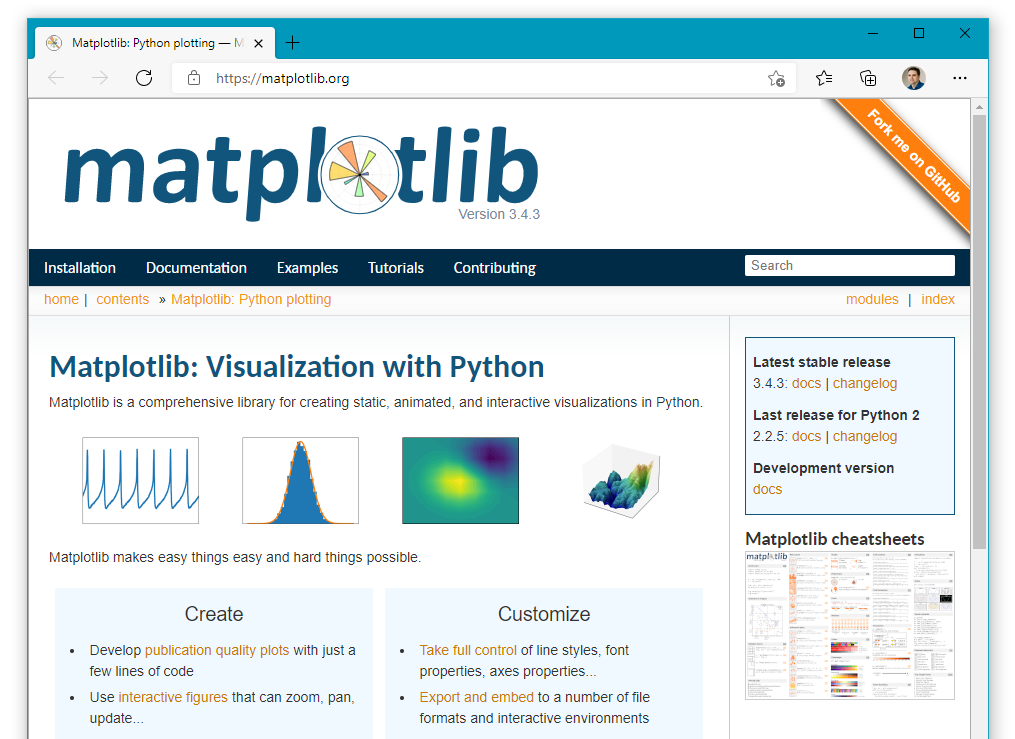
\includegraphics[scale=0.32]{image/matplotlib.png}} \\
\vspace{0.3cm}
\href{https://matplotlib.org/}{\beamerbutton{Открыть}}
\end{frame}

\subsection{Установка библиотеки}
\begin{frame}{Библиотека matplotlib}
\textbf{\# Установка библиотеки matplotlib} \\
\vspace{0.5cm}
pip install matplotlib
\end{frame}

\begin{frame}{Основные компоненты matplotlib}

\begin{minipage}{0.35\textwidth}
  \begin{flushleft}
	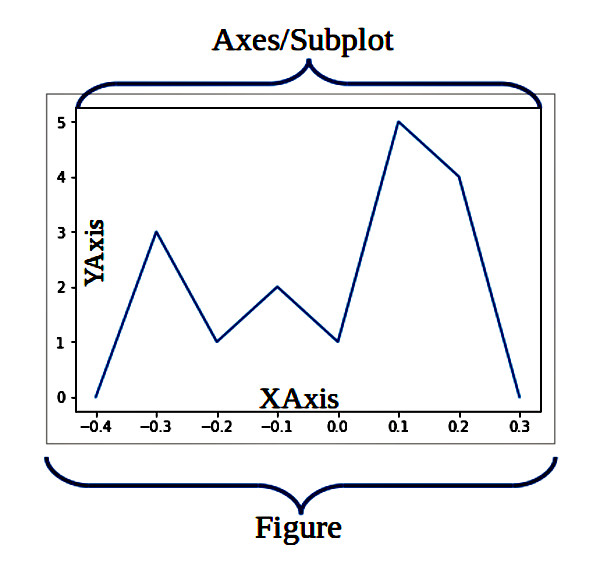
\includegraphics[scale=0.2]{image/mpl_anatomy.jpg}
	\vspace{2.2cm}
  \end{flushleft}
\end{minipage}
\begin{minipage}{0.6\textwidth}
  \begin{flushright}  
	\begin{itemize}
		\item \textbf{Figure} -- контейнер самого верхнего уровня, которых может содержать несколько контейнеров \textit{Axes}. 
		\item \textbf{Axes} -- область на которой отражаются графики, а так же все вспомогательные атрибуты (линии сетки, метки, указатели и т.д.).
		\item Каждая область \textbf{Axes} содержит \textbf{XAxis} и \textbf{YAxis}, которые в свою очередь содержат: деления, метки и прочие вспомогательные атрибуты. 
\end{itemize}
  \end{flushright}
\end{minipage}

\end{frame}



\subsection{Вывод графика}
\begin{frame}{Вывод графика}
\lstinputlisting[language=Python]{code_04/41.py}
\vspace{0cm}
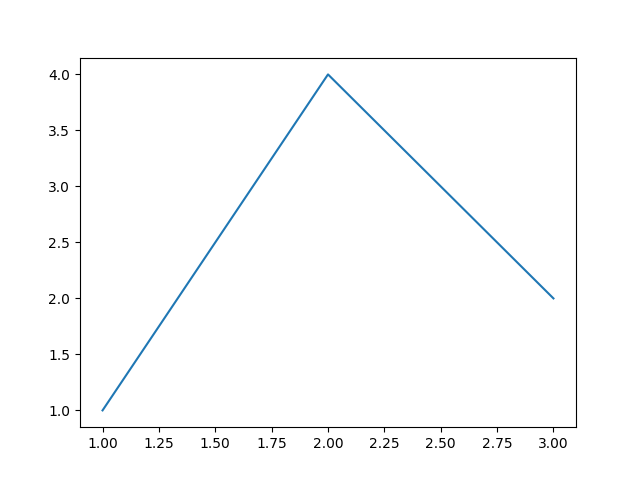
\includegraphics[scale=0.35]{code_04/41.png}
\end{frame}


\begin{frame}{Заголовок, подписи, легенда}
\lstinputlisting[language=Python]{code_04/42_1.py}
\vspace{0cm}
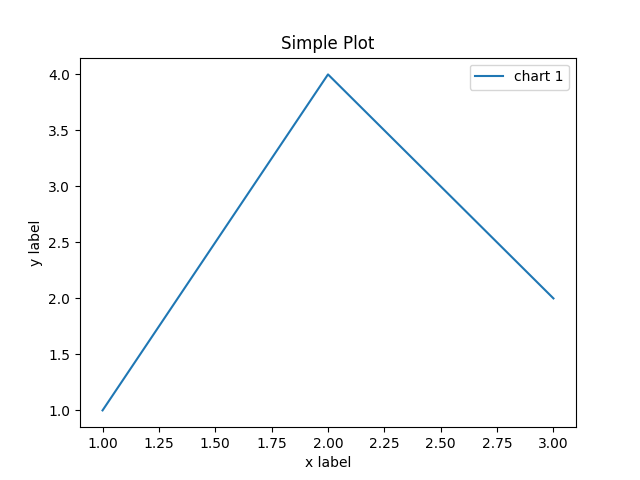
\includegraphics[scale=0.35]{code_04/42.png}
\end{frame}

\begin{frame}{Два и более графиков}
\lstinputlisting[language=Python]{code_04/43_1.py}
\vspace{0cm}
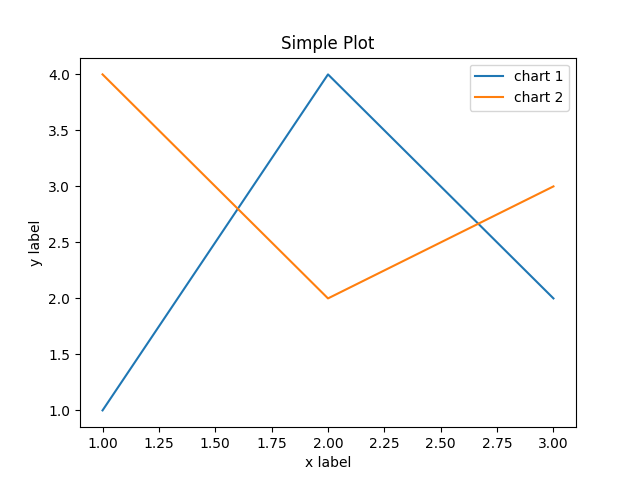
\includegraphics[scale=0.35]{code_04/43.png}
\end{frame}

\begin{frame}{Сетка}
\lstinputlisting[language=Python]{code_04/44_1.py}
\vspace{0cm}
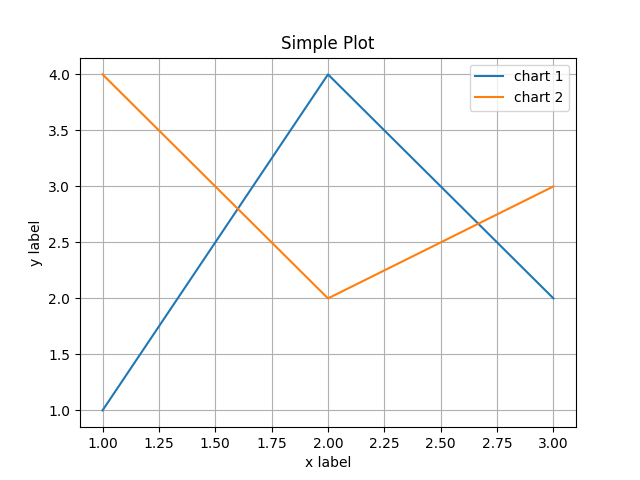
\includegraphics[scale=0.35]{code_04/44.png}
\end{frame}


\section{Математическая библиотека numpy}
\begin{frame}[t]{Оглавление}
\tableofcontents[currentsection]
\end{frame}

\subsection{Установка библиотеки}
\begin{frame}{Библиотека numpy}
\textbf{\# Установка библиотек} \\
\vspace{0.5cm}
pip install numpy \\
\vspace{0.2cm}
pip install scipy \\
\vspace{0.5cm}

\textbf{NumPy} -- библиотека поддержки многомерных массивов (включая матрицы) и высокоуровневых математических функций, предназначенных для работы с многомерными массивами. NumPy можно рассматривать как свободную альтернативу MATLAB.

\vspace{0.5cm}
\textbf{SciPy} -- библиотека для выполнения научных и инженерных расчётов. 

\end{frame}


\begin{frame}{График функции y = sin(x)}
\lstinputlisting[language=Python]{code_04/45.py}
\end{frame}


\begin{frame}{График функции y = sin(x)}
\lstinputlisting[language=Python]{code_04/56.py}
\end{frame}

\begin{frame}{Матрицы}
\textbf{Матрицей} в математике называют объект, записываемый в виде прямоугольной таблицы, элементами которой являются числа (могут быть как действительные, так и комплексные). \\
\vspace{0.5cm}
\[
  A_{3\times 3} = 
  \begin{pmatrix}
    a_{11} & a_{12} & a_{13}\\
    a_{21} & a_{22} & a_{23}\\
    a_{31} & a_{32} & a_{33}
  \end{pmatrix}
\]

\begin{itemize}
\item Матрица состоит из i-строк и j-столбцов;
\item Каждый ее элемент имеет соответствующее позиционное обозначение: $a_{ij}$ находится на \emph{i}-ой строке и \emph{j}-м столбце;
\item Главная диагональ -- элементы, у которых совпадают номера строк и столбцов.
\end{itemize}
\end{frame}

\subsection{Вектор}
\begin{frame}{Вектор}
\textbf{Вектором} называется матрица, у которой есть только один столбец или одна строка. \\
\vspace{0.5cm}
Вектор-строка имеет следующую математическую запись
\vspace{0.2cm}
\[
  v = 
  \begin{pmatrix}
    a_{11} & a_{12} \\
  \end{pmatrix}
\]
\\
\vspace{0.2cm}
в Python можно задать следующим образом
\vspace{0.2cm}
\lstinputlisting[language=Python]{code_04/47.py}
\vspace{0.2cm}
Результат: \\
\lstinputlisting[language=Python]{code_04/47_1.txt}
\end{frame}


\begin{frame}{Вектор}
Вектор-столбец имеет следующую математическую запись
\vspace{0.2cm}
\[
  v = 
  \begin{pmatrix}
    a_{11}\\
    a_{21}\\
  \end{pmatrix}
\]
\\
\vspace{0.2cm}
в Python можно задать следующим образом
\vspace{0.2cm}
\lstinputlisting[language=Python]{code_04/48.py}
\vspace{0.2cm}
Результат: \\
\lstinputlisting[language=Python]{code_04/48_1.txt}
\end{frame}


\subsection{Квадратная матрица}
\begin{frame}{Квадратная матрица}
Матрица называется \textbf{квадратной}, если количество строк и столбцов совпадают.
\vspace{0.2cm}
\[
  v = 
  \begin{pmatrix}
    1 & 2 & 3 \\
    4 & 5 & 6 \\
    7 & 8 & 9 \\
  \end{pmatrix}
\]
\\
%\vspace{0.2cm}
\lstinputlisting[language=Python]{code_04/49.py}
%\vspace{0.2cm}
Результат: \\
\lstinputlisting[language=Python]{code_04/49_1.txt}
\end{frame}


\subsection{Диагональная матрица}
\begin{frame}{Диагональная матрица}
\textbf{Диагональная матрица} – матрица, у которой все элементы, кроме тех, что расположены на главной диагонали, равны нулю.
\vspace{0.2cm}
\[
  v = 
  \begin{pmatrix}
    1 & 0 & 0 \\
    0 & 5 & 0 \\
    0 & 0 & 9 \\
  \end{pmatrix}
\]
\\
%\vspace{0.2cm}
\lstinputlisting[language=Python]{code_04/50.py}
%\vspace{0.2cm}
Результат: \\
\lstinputlisting[language=Python]{code_04/50_1.txt}
\end{frame}

\subsection{Единичная матрица}
\begin{frame}{Единичная матрица}
\textbf{Единичной матрицей} называют такую квадратную матрицу, у которой элементы главной диагонали равны единицы, а все остальные нулю.
\vspace{0.2cm}
\[
  v = 
  \begin{pmatrix}
    1 & 0 & 0 \\
    0 & 1 & 0 \\
    0 & 0 & 1 \\
  \end{pmatrix}
\]
\\
\vspace{-0.6cm}
\lstinputlisting[language=Python]{code_04/51.py}
%\vspace{0.2cm}
Результат: \\
\lstinputlisting[language=Python]{code_04/51_1.txt}
\end{frame}


\subsection{Сложение матриц}
\begin{frame}{Сложение матриц A + B}
\[
  A = 
  \begin{pmatrix}
    a_{11} & a_{12} & a_{13}\\
    a_{21} & a_{22} & a_{23}\\
    a_{31} & a_{32} & a_{33}
  \end{pmatrix}
\]
\\
\[
  B = 
  \begin{pmatrix}
    b_{11} & b_{12} & b_{13}\\
    b_{21} & b_{22} & b_{23}\\
    b_{31} & b_{32} & b_{33}
  \end{pmatrix}
\]
\\
\vspace{0.5cm}
Сложение матриц A + B
\\
\[
  A + B = 
  \begin{pmatrix}
    a_{11} + b_{11} & a_{12} + b_{12} & a_{11} + b_{13}\\
    a_{21} + b_{21} & a_{22} + b_{22} & a_{23} + b_{23}\\
    a_{31} + b_{31} & a_{32} + b_{32} & a_{33} + b_{33}
  \end{pmatrix}
\]
\end{frame}


\begin{frame}{Сложение матриц A + B}
\lstinputlisting[language=Python]{code_04/53.py}
%\vspace{0.2cm}
Результат: \\
\lstinputlisting[language=Python]{code_04/53_1.txt}
\end{frame}


\subsection{Вычитание матриц}
\begin{frame}{Вычитание матриц A - B}
\[
  A = 
  \begin{pmatrix}
    a_{11} & a_{12} & a_{13}\\
    a_{21} & a_{22} & a_{23}\\
    a_{31} & a_{32} & a_{33}
  \end{pmatrix}
\]
\\
\[
  B = 
  \begin{pmatrix}
    b_{11} & b_{12} & b_{13}\\
    b_{21} & b_{22} & b_{23}\\
    b_{31} & b_{32} & b_{33}
  \end{pmatrix}
\]
\\
\vspace{0.5cm}
Вычитание матриц A - B
\\
\[
  A - B = 
  \begin{pmatrix}
    a_{11} - b_{11} & a_{12} - b_{12} & a_{11} - b_{13}\\
    a_{21} - b_{21} & a_{22} - b_{22} & a_{23} - b_{23}\\
    a_{31} - b_{31} & a_{32} - b_{32} & a_{33} - b_{33}
  \end{pmatrix}
\]
\end{frame}


\begin{frame}{Вычитание матриц A - B}
\lstinputlisting[language=Python]{code_04/54.py}
%\vspace{0.2cm}
Результат: \\
\lstinputlisting[language=Python]{code_04/54_1.txt}
\end{frame}


\part{2}
\subsection{Скалярное произведение}
\begin{frame}{Скалярное произведение A $\times$ n}
В скалярном произведении постоянное значение умножается на каждый элемент матрицы.\\
\[
  A = 
  \begin{pmatrix}
    a_{11} & a_{12} & a_{13}\\
    a_{21} & a_{22} & a_{23}\\
    a_{31} & a_{32} & a_{33}
  \end{pmatrix}
\]
\\
\vspace{0.5cm}
Умножения матрицы А на число \emph{n}
\\
\[
  A \times n = 
  \begin{pmatrix}
    a_{11} \times n & a_{12} \times n & a_{11} \times n \\
    a_{21} \times n & a_{22} \times n & a_{23} \times n \\
    a_{31} \times n & a_{32} \times n & a_{33} \times n
  \end{pmatrix}
\]
\end{frame}


\begin{frame}{Скалярное произведение  A $\times$ n}
Оператор $*$ используется для умножения скалярного значения на элементы входной матрицы.
\vspace{0.2cm}
\lstinputlisting[language=Python]{code_04/55.py}
%\vspace{0.2cm}
Результат: \\
\lstinputlisting[language=Python]{code_04/55_1.txt}
\end{frame}


\subsection{Скалярное деление}
\begin{frame}{Скалярное деление A / n}
В скалярном деление каждый элемент матрицы делиться на постоянное значение.\\
\[
  A = 
  \begin{pmatrix}
    a_{11} & a_{12} & a_{13}\\
    a_{21} & a_{22} & a_{23}\\
    a_{31} & a_{32} & a_{33}
  \end{pmatrix}
\]
\\
\vspace{0.5cm}
Деление матрицы А на число \emph{n}
\\
\[
  A / n = 
  \begin{pmatrix}
    a_{11} / n & a_{12} / n & a_{11} / n \\
    a_{21} / n & a_{22} / n & a_{23} / n \\
    a_{31} / n & a_{32} / n & a_{33} / n
  \end{pmatrix}
\]
\end{frame}


\begin{frame}{Скалярное деление A / n}
Оператор ‘/’ делит каждый элемент матрицы на скалярное / постоянное значение.
\vspace{0.2cm}
\lstinputlisting[language=Python]{code_04/57.py}
%\vspace{0.2cm}
Результат: \\
\lstinputlisting[language=Python]{code_04/57_1.txt}
\end{frame}


\subsection{Произведение матриц}
\begin{frame}{Произведение матриц A $\times$ B}
\[
  A = 
  \begin{pmatrix}
    a_{11} & a_{12} \\
    a_{21} & a_{22} 
  \end{pmatrix} 
\]
\\
\[
  B = 
  \begin{pmatrix}
    b_{11} & b_{12} \\
    b_{21} & b_{22} 
  \end{pmatrix}
\]
\\
\vspace{0.5cm}
Произведение матриц A $\times$ B
\\
\[
  A \times B = 
  \begin{pmatrix}
    a_{11} \times b_{11} + a_{12} \times b_{21} & a_{11} \times b_{12} + a_{12} \times b_{22} \\
    a_{21} \times b_{11} + a_{22} \times b_{21} & a_{21} \times b_{12} + a_{22} \times b_{22} 
  \end{pmatrix}
\]
\end{frame}


\begin{frame}{Произведение матриц A $\times$ B}
\lstinputlisting[language=Python]{code_04/52.py}
%\vspace{0.2cm}
Результат: \\
\lstinputlisting[language=Python]{code_04/52_1.txt}
\end{frame}


\subsection{Транспонирование матрицы}
\begin{frame}{Транспонирование матрицы}
Транспонирование матрицы включает в себя переворачивание матрицы по соответствующим диагоналям, т. е. меняются местами строки и столбцы входной матрицы.
\vspace{0.5cm}
\[
  A = 
  \begin{pmatrix}
    a_{11} & a_{12} & a_{13} \\
    a_{21} & a_{22} & a_{23}
  \end{pmatrix} 
\]
\\
После выполнения операции транспонирования Matrix.T
\\
\[
  A = A.T = 
  \begin{pmatrix}
    a_{11} & a_{21} \\
    a_{12} & a_{22} \\
    a_{13} & a_{23} 
  \end{pmatrix}
\]
\end{frame}


\begin{frame}{Транспонирование матрицы}
\lstinputlisting[language=Python]{code_04/58.py}
%\vspace{0.2cm}
Результат: \\
\lstinputlisting[language=Python]{code_04/58_1.txt}
\end{frame}


\begin{frame}{Литература}
\begin{columns}[onlytextwidth,T]
    \column{30mm}
	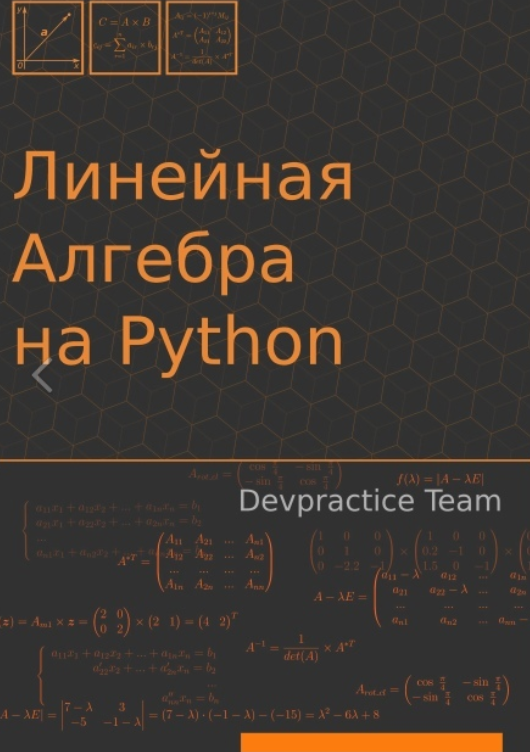
\includegraphics[scale=0.4]{image/math_pybook.png}
    \column{\dimexpr\linewidth-30mm-20mm}
	Devpractice Team. \\Линейная алгебра на Python [2019]         
    \end{columns}  
\end{frame}


\part{3}

\begin{frame}[t]{Литература}
\setbeamertemplate{bibliography item}[text]

\begin{thebibliography}{3}

\bibitem{src_this}
Презентация [Лекции 01-04] \\
\vspace{0.2cm}
\textit{\href{https://github.com/IRyazantsev/mpei_python_mini-course_2021/tree/main/bin}{https://github.com/IRyazantsev/mpei\_python\_mini-course\_2021/tree/main/bin}}

\bibitem{texbook}
Python 3. Самое необходимое | Дронов В.А., Прохоренок Н.А.

\bibitem{texbook} 
Изучаем Python. Том 1, 2 | Лутц Марк

\bibitem{texbook} 
Python 3 и PyQt 5. Разработка приложений | Прохоренок Н.А., Дронов В.А.

\bibitem{texbook} 
Django 3.0. Практика создания веб-сайтов на Python | Дронов В. А.

\bibitem{texbook} 
Разработка веб-приложений с использованием Flask | Гринберг Мигель

\end{thebibliography}
\end{frame}


\begin{frame}[t]{Вопросы}
\vspace{0.7cm}
\center{
\includegraphics[scale=0.3]{image/questions.jpg}} \\
\end{frame}

\end{document}